\begin{figure}
\begin{floatrow}
	\ffigbox{
		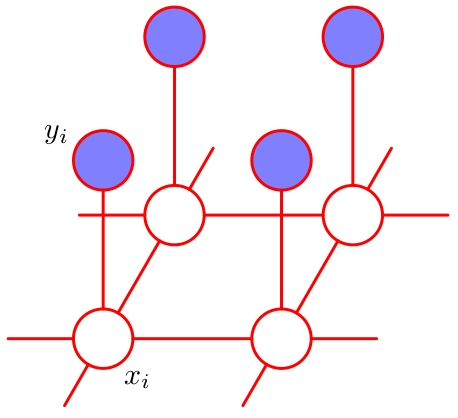
\includegraphics[width=.3\textwidth]{resources/crf}
	}{
		\caption{An undirected graph, representing the graph that was used for
		modeling our Conditional Random Field}
		\label{fig:crf}
	}
	\capbtabbox{%
		\begin{tabular}{@{\extracolsep{4pt}}l r r r r @{}}
		\hline
		 & \multicolumn{2}{c}{\emph{Pre-trained}} & \multicolumn{2}{c}{\emph{Direct}} \\
		 \cline{2-3} \cline{4-5}
		  & \textbf{Image} & \textbf{Text} & \textbf{Image} & \textbf{Text} \\
		\textbf{Precision} & 0.269 & 0.979 & 0.241 & 0.979 \\
		\textbf{Recall} & 0.743 & 0.854 &  0.750 & 0.830 \\
		\textbf{F-score} & 0.395 & 0.912 & 0.365 & 0.898 \\\hline
		\end{tabular}
	}
	{
		\caption{scores for image localization}
		\label{tab:imagelocresults}
	}
\end{floatrow}
\end{figure}
A CRF provides the labelling for an undirected graph. In this case, a grid was
used, shaped as figure \ref{fig:crf}, where $y_i$ is the percieved data for an
image patch, and $x_i$ is the label assigned to that patch by the learning
algorithm. The ultimate goal is to find the labelling for $\mathbf{x}$ that
minimizes the loss function. 

For calculating this loss function, the CRF has an energy function for each pair
$\{x_i, y_y\}$, a simple
example of which, taken from \cite{bishop2006pattern}\footnote{This example is actually
used in an example of Markov Random Fields, but this specific graph is
comparable to a CRF},  has the following form: 
\begin{equation}
E(\mathbf{x}, \mathbf{y}) = h\sum_i x_i - \beta \sum_{\{i, j\}} x_i x_j
- \eta \sum_i x_i y_i
\end{equation}
In this energy function, $\eta$ is a positive constant. The product $\eta \sum_i
x_i y_i$ will then be of a greater number when $x_i$ and $y_i$ are similar.
$\beta$ is another positive constant, which, in combination with the sum of
products $x_i x_j$ should result in higher energy when the neigbouring nodes
$x_j$ have a similar value to $x_i$. Finally $h$ is a constant that can be used
to bias the energy function to either one of the classes, for example when
dealing with an unfair distribution like ours. Various implementations of
Conditional Random Fields might use various types of energy function, but the
idea is the same.

Finding the solution with maximum energy is not trivial, since 
looping over all possible solutions and selecting the one with the highest energy
for all nodes would quickly become intractable. Therefore a solver should be
used, in this case the SSVM.

\todo{Explain the SSVM}

\todo{Explain different types of processing: preprocessed with SVM and with
either 1 or 4 HOGs per image patch}
\todo{Explain two-stage validation. Also explain why we can compare the scores
of the different SVM's (the question jan van Gemert asked)}
